\documentclass[12pt]{report}
\usepackage[print,nopanel]{pdfscreen}
%\begin{print}
\usepackage{lipsum}% http://ctan.org/pkg/lipsum
\usepackage{titletoc}% http://ctan.org/pkg/titletoc
%\section{type}
%\usepackage{sagetex}

\usepackage{listings}
\bibliographystyle{ieeetr}

\usepackage{lastpage}
\usepackage{macro/macro}
\usepackage{float}
\usepackage{fancyhdr}
\usepackage{verbatim}
\usepackage[Glenn]{fncychap}
\lhead{\bfseries OpenSCAD's Customizer}
\rhead{}
\usepackage[left=2.5cm, right=1.5cm, top=1.5cm, bottom=1.5cm]{geometry}
\pagestyle{fancy}
%\end{print}
\margins{2.5cm}{1.5cm}{1.5cm}{1.5cm}
\begin{screen}

\renewcommand{\encodingdefault}{T1}
\usepackage{setspace}
\linespread{1.5}
\renewcommand{\rmdefault}{ptm}
\end{screen}
\screensize{8cm}{9cm}
\overlay{overlay8.pdf}
\usepackage{graphicx}

\begin{document}
\newcommand{\centertext}[1]{\begin{center}\textbf{#1}\end{center}}
\newcommand{\student}{\vskip 2.5cm}
\newcommand{\supervisor}{\vskip 2cm}
\newcommand{\stamp}{\vskip 2.5cm}
\newcommand{\HRule}{\rule{\linewidth}{0.5mm}}
\newcommand{\projecttitle}{ \fontsize{24}{25}\selectfont \bf{Multi-Threaded Geometric Rendering}}
\newcommand{\tab}[1]{\hspace{.4\textwidth}\rlap{#1}}
\newcommand{\itab}[1]{\hspace{.05\textwidth}\rlap{#1}}
\newcommand{\logo}[1]{\includegraphics[scale=0.16]{#1}}
\newcommand{\submitted}{
\vskip 0.2in
\textnormal{ {\fontsize{14}{16}\selectfont \textbf{Project Report}} \\
	{\fontsize{12}{13}\selectfont of Major Project}\\
}
\vskip 0.2in

\textnormal{
 {\fontsize{14}{16}\selectfont \textbf{Bachelor of Technology}\\}
 {\fontsize{16}{17}\selectfont  (Computer Science and Engineering)\\}
}
\vskip 4cm
%\logo{images/gne.png}
%\image{0.7}{images/gne.png}{}

\includegraphics[width=7cm]{images/gne.png}
\vskip 2cm
\begin{minipage}{0.4\textwidth}
\begin{flushleft} \large
{Submitted by:}\\
\textnormal{{\fontsize{12}{13}\selectfont Amarjeet Singh Kapoor\\ D4CSE 2013-17 \\135005\\1311017 \\}} % Your name
\end{flushleft}
\end{minipage}
~
\begin{minipage}{0.4\textwidth}
\begin{flushright}
\textnormal{ \\
	 {\fontsize{12}{13}\selectfont Govind Sharma\\ D4CSE 2013-17 \\135026\\1311053\\}} % Supervisor's Name
\end{flushright}
\end{minipage}\\[1.5cm]
\HRule \\[0.4cm]

\textnormal{
Guru Nanak Dev Engineering College \\
Ludhiana 141006}
}


\newcommand{\pagetitle}{\begin{center}
\projecttitle
\Large\textbf{}\\
\submitted
\vskip 1cm

\end{center}}
\newcommand{\openoffice}{\textbf{OpenOffice}}
\newcommand{\frontmatter}[1]{\begin{Large} \textbf{#1} \end{Large}}
\newcommand{\ppttitle}{\begin{center}
\end{center}}

\begin{screen}
\ppttitle
\end{screen}

\thispagestyle{empty} 
\pagetitle
\newpage
\pagenumbering{Roman}
\cfoot{\thepage}

\begin{Large}
\centertext{Abstract}
\end{Large}


User Interface for Customizing Models in OpenSCAD is the project that I worked upon for my 6-month training and also as Google summer of code project. It is under the umbrella organization of BRL-CAD. OpenSCAD is an open source organization that serves a free software to create solid 3d CAD objects. OpenSCAD has in a way redefined how easy 3D modeling can be. But the Wikipedia article on OpenSCAD says that it is a non-interactive modeler, but rather a 3D compiler based on a textual description language. Pay attention to the above line, it’s primarily what I’ll be talking about.

What the guys over at Wikipedia said is true but their version of the truth needs a little filtration (rather trimming). OpenSCAD’s way of customization is interactive, just not through a graphical interface. And this contingency makes the whole 3D modeling thing a little less easy than it can be. But all of that is about to change.

Solid 3D modeling. That sounds like some serious business. But it’s just an awesome tool for making models pertaining to many uses (mostly 3D printing). And 3D printing as we can all agree upon is cool. 3D models can be created by anyone using OpenSCAD. OpenSCAD is as much for designers as it is for you and me. What else can most people agree upon apart from the fact that solid 3D modeling is cool? A graphical interface is simpler and more intuitive to use. There is a general aversion for typing commands in order to get things done. Simply put, more people have an inclination towards GUI.

This is something that OpenSCAD lacked. But the benevolent folks at Thingiverse.com found a way to help out the demographic intersection of GUI lovers and OpenSCAD users. The website provides an easy to use interface to customize models of OpenSCAD. All one needs to do is upload the OpenSCAD file. After uploading the file, what you’ll see can only be described as being magic. I’m kidding, it’s just very useful is all. The OpenSCAD’s script is used to make a form containing slide bars, text boxes, combo boxes, labels, etc all for the singular purpose of customizing models.

My project was to include similar functionality into OpenSCAD itself. Constantly having to upload files created in one software (OpenSCAD) to a website in order to customize your models can get a little problematic as one is uploading scripts without being able to confirm how the script will translate into a form on the site. Wouldn’t it be great if everything is at one place, the original place: OpenSCAD? Of course, it would.

My project intends to define a user interface to customize models interactively instead of having to modify them manually. It will enable the user to create the templates for a given model which can further be changed as per user’s requirements.

This project will allow the modelers to create generic models (templates) which others can then customize to cater to their own use.
\newpage
\begin{Large}
\centertext{Acknowledgement}
\end{Large}

I, student of Guru Nanak Dev Engineering College, Ludhiana, have taken efforts in this project.
However, it would not have been possible without the kind support and help of many individuals
and organizations. I would like to extend my sincere thanks to all of them.\\

The author is highly grateful to Dr. M.S. Saini Director, Guru Nanak Dev Engineering College, Ludhiana for providing him with the opportunity to carry out his Six Weeks Training at
Testing and Consultancy Cell, Guru Nanak Dev Engineering College, Ludhiana.\\

The author would like to whole heartedly thank Dr. H.S. Rai Dean, Testing and Consultancy
Cell, Guru Nanak Dev Engineering College, Ludhiana who is a vast sea of knowledge and without whose constant and never ending support and motivation, it would never have been possible to complete the project and other assignments so efficiently and effectively.\\

Finally, I would thanks My Mentors at OpenSCAD organisation Marius Kintel and Torsten Paul. Without their encouragementand Guidence it would not have been possible to complete this project
in such an efficient manner.


\vskip 1.0cm 
\noindent Amarjeet Singh Kapoor


\newpage
\tableofcontents
\newpage
\listoffigures
\newpage
\listoftables
\newpage


\pagenumbering{arabic}
\cfoot{\thepage}

\newpage
\chapter{INTRODUCTION OF ORGANIZATION}
\begin{figure}[ht]
\centering
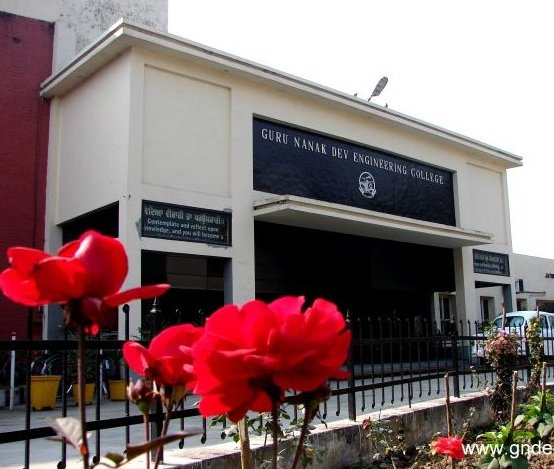
\includegraphics[scale=0.5]{images/gndec.jpg}
\caption{Guru Nanak Dev Engineering College}
\end{figure}
\hspace{-1.7em} I had my Six Month Industrial Training at TCC-Testing And Consultancy Cell, GNDEC Ludhiana. Guru Nanak Dev Engineering College was established by the Nankana
Sahib Education Trust Ludhiana. The Nankana Sahib Education Trust i.e NSET
was founded in memory of the most sacred temple of Sri Nankana Sahib, birth place
of Sri Guru Nanak Dev Ji. With the mission of Removal of Economic Backwardness
through Technology Shiromani Gurudwara Parbandhak Committee i.e SGPC started a
Poly technical was started in 1953 and Guru Nanak Dev Engineering College was established in 1956.\\


The main goal of this institute is:
\begin{itemize}
\item To build and promote teams of experts in the upcoming specialisations.
\item To promote quality research and undertake research projects keeping in view their
relevance to needs and requirements of technology in local industry.
\item To achieve total financial independence.
\item To start online transfer of knowledge in appropriate technology by means of establishing multipurpose resource centres.
\end{itemize}
\section{Testing and Consutancy Cell}

I had my Six Month Institutional Training at TCC i.e Testing And
Consultancy Cell,
GNDEC Ludhiana under the guidance of Dr. H.S.Rai Dean Testing and Consultancy Cell.
Testing and Consultancy Cell was established in the year 1979 with a basic aim to produce
quality service for technical problems at reasonable and affordable rates as a service to society
in general and Engineering fraternity in particular.\\
\begin{figure}[ht]
\centering
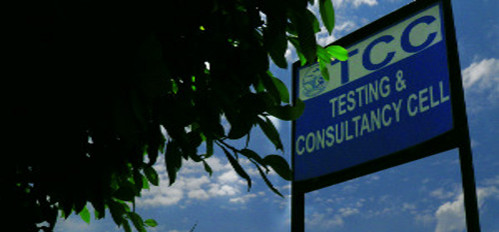
\includegraphics[scale=0.7]{images/aw.jpg}
\caption{Testing and Consultancy Cell}
\end{figure}
\hspace{-1.7em} 

Consultancy Services are being rendered by various Departments of the College to the
industry, Sate Government Departments and Entrepreneurs and are extended in the form of
expert advice in design, testing of materials \& equipment, technical surveys, technical audit,
calibration of instruments, preparation of technical feasibility reports etc.
This consultancy cell of the college has given a new dimension to the development
programmers of the College. Consultancy projects of over Rs. one crore are completed by the
Consultancy cell during financial year 2009-10. \\

Ours is a pioneer institute providing Consultancy Services in the States of Punjab, Haryana,
Himachal, J\&K and Rajasthan. Various Major Clients of the Consultancy Cell are as under:\\
\begin{itemize}
\item Northern Railway, Govt. of India
\item Indian Oil Corporation Ltd.
\item Larson \& Turbo.
\item Multi National Companies like AFCON \& PAULINGS.
\item Punjab Water Supply \& Sewage Board
\end{itemize}


\newpage


\chapter{Introduction To Project}

\section{Overview}

\begin{figure}[H] 
	\centering 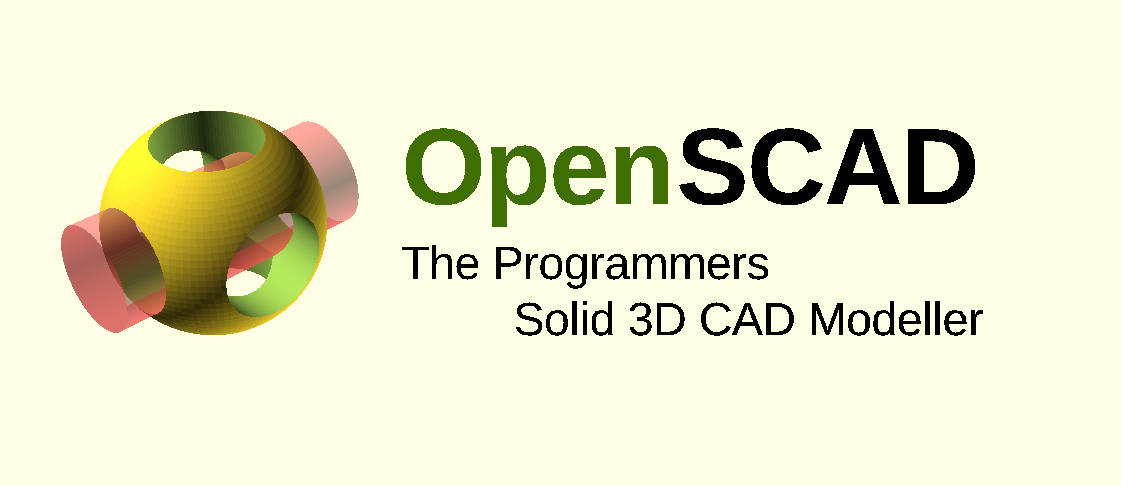
\includegraphics[scale=0.31]{images/openscad.png}
	\caption{OpenSCAD's logo}
	\label{fig:openscadlogo}
\end{figure}

User Interface for Customizing Models in OpenSCAD is the project that I worked upon for my 6 month training. It is under the umbrella organization of BRL-CAD. OpenSCAD is a free and Open source software application for creating solid 3D CAD objects. It is a script only based modeller, with a specific description language. Parts cannot be selected or modified by mouse in the 3D view. An OpenSCAD script specifies geometric primitives and defines how they are modified and manipulated to render a 3D model. OpenSCAD is available for Windows, Linux and OS X. It does constructive solid geometry (CSG).

OpenSCAD has in a way redefined how easy 3D modeling can be. But the Wikipedia article on OpenSCAD says that it is a non interactive modeler, but rather a 3D compiler based on a textual description language. Pay attention to the above line, it’s primarily what I’ll be talking about.

Solid 3D modeling. That sounds like some serious business. But it’s just an awesome tool for making models pertaining to many uses (mostly 3D printing). And 3D printing as we can all agree upon is cool. 3D models can be created by anyone using OpenSCAD. OpenSCAD is as much for designers as it is for you and me. What else can most people agree upon apart from the fact that solid 3D modeling is cool? A graphical interface is simpler and more intuitive to use. There is a general aversion for typing commands in order to get things done. Simply put, more people have an inclination towards GUI.

This is something that OpenSCAD lacked. But the benevolent folks at Thingiverse.com found a way to help out the demographic intersection of GUI lovers and OpenSCAD users. The website provides an easy to use interface to customize models of OpenSCAD. All one needs to do is upload the OpenSCAD file. After uploading the file, what you’ll see can only be described as being magic. I’m kidding, it’s just very useful is all. The OpenSCAD’s script is used to make a form containing slide bars, text boxes, combo boxes, labels, etc all for the singular purpose of customizing models.

My project was to include similar functionality into OpenSCAD itself. Constantly having to upload files created in one software (OpenSCAD) to a website in order to customize your models can get a little problematic as one is uploading scripts without being able to confirm how the script will translate into a form on the site. Wouldn’t it be great if everything is at one place, the original place: OpenSCAD? Of course, it would.

My project intends to define a user interface to customize models interactively instead of having to modify them manually. It will enable the user to create the templates for a given model which can further be changed as per user’s requirements.

This project will allow the modelers to create generic models (templates) which others can then customize to cater to their own use.

This project is based on the User interface of OpenSCAD Software. The main idea of this project is to provide users with features to change certain variables or parameters in .scad file using form like interface which may include slide bar, check box, text box, ranges etc. so that we can visualize the changes in output on the basis of input side by side instead of manually changing different parameters. It will help the user able to create the templates for given model which can further be changed as per user's requirements. 

The core part of this project is implemented using C++, flex and bison and for GUI part Qt is used. Apart for that Make, qmake and cmake are used for making project and test cases.
Testing is done using the travis and ctest. Github is used to manage code and IRC to communicate with the mentors.
  
My training being not based on particular language or technology, different type of open-source softwares and technologies are 
used in this project and many during my training which are not used in this 
project like android, ejabberd (server bassed on erlang and XMPP protcol) for\emph{ sunehaG} and GRASS GIS, python, shell scripting for \emph{The Road Project}.

\section{The Existing System}
The only System exiting to solve above problem is Thingiverse's Customizer which allows you to design parametric objects that can be customized with an easy web interface. They currently support OpenSCAD designs. Just upload your OpenSCAD script to Thingiverse and then anyone can open it in Customizer and customize it. Also, if you tag your Thing with the "customizer" tag, then your Thing page will automatically display an Open In Customizer button as a shortcut. 

But there syntax is little messy as they use comments to generate customizer which also limits the useablitiy of the customizer. \\

{\bf {Limitations of previous system }}
\begin{itemize}
\item \emph{Not supported by OpenSCAD offically.}

\item Doesn't work in combination with OpenSCAD software

\item Works only in online mode

\item No Command-line Support 

\item Based upon string processing not on lexical anylises. 

\item No internal support.

\item Commplex work flow.

\item Scripts must have all the code they need in a single .scad file

\item You could only put one .scad file in your Thingiverse entry
\end{itemize}

\section{User Requirement Analysis}
User Requirements Analysis for a software system is a complete description of the requirements of the User. It includes functional Requirements
and Non-functional Requirements. Non-functional requirements are
requirements which impose constraints on the design or implementation.

 
{\bf Users of the System:}
    \begin{enumerate}
        \item Modeler: Modelers are the people how the code to create model theirs for their own use or for commercial use.
        \item Client: These are the people which will customize model to their need made by modelers before ordering or printing model themselves.
        \item Other Softwares: Many web Apps or other software using OpenSCAD as there Backend might need to interact with the customizer.
               
    \end{enumerate}

\subsection{Functional Requirements}
\begin{itemize}
    \item {\bf Syntax to generate a widget to modify parameter}: This means there should be a syntax which could be used to generate a different widget for a different type of parameters.
    The widgets that we intend to support are:
    \begin{enumerate}
        \item Spinbox
            \begin{enumerate}
                \item With Increment Size
                \item Without Increment Size
            \end{enumerate}
        \item Checkbox
        \item Slider
            \begin{enumerate}
                \item With Increment Size
                \item With Default Increment Size
            \end{enumerate}
        \item Textbox
        \item Special vector
        \item Combo Box
            \begin{enumerate}
                \item Simple
                \item Labeled
            \end{enumerate}
   
    \begin{table}[h]
        \centering
        \caption{Table to show the required support of widgets for different DataType}
        \begin{tabular}{ |c|c|c|c|c|c| }
            \hline
            & \multicolumn{5}{|c|}{Type of Widgets} \\
            \hline
            Type of Data&    Number&    String&    BOOL &Vector &Range     \\ [0.5ex]
            \hline
            SpinBox&Y&    -&    -&    -&    - \\ \hline
            ComboBox&    Y&    Y&    -&    -&    - \\ \hline
            Text&    Y&    Y&    -&    O&    - \\ \hline
            Slider&    Y&    -&    -&    -&    - \\ \hline
            Checkbox&    -&    -&    Y&    -&    - \\ [1ex]
            \hline
        \end{tabular}
        \label{table2}
    \end{table}
   
    \end{enumerate}
    \item {\bf Syntax to Describe parameter}:
        This means there should be a syntax which could be used to provide a description for the parameter.
    \item \textbf{Syntax to Group Parameter}:
        This means there should be a syntax which could be used to group the parameters into different groups or tab to easily manage Customizer and make customizer interface little simple.
    \item \textbf{Syntax to Hide parameters}
        This means there should be a syntax which could be used to Hiding certain parameters.
    \item \textbf{Syntax to make certain parameters Global}
        This means there should be a syntax which could be used to make certain parameters global i.e. they are present in each and every group.
    \item \textbf{Save the set of parameters in JSON file}:
    This feature means there should be a way a way that gives user the ability to save the value of the parameter and also we can apply them through the cmd-line and get the output.
   
    \item \textbf{Provide GUI to add Set of Parameters}
        This means there should be a way to store different set of parameters which represent different models from generic model.
    \end{itemize}
\subsection{Non-functional requirements}
\begin{enumerate}
    \item Extensible: It should be able to support future functional requirements
    \item Usability: Simple user interfaces that a layman can understand.
    \item Modular Structure: The software should have  structure. So, that different parts of software would be changed without affecting other parts.
 
\end{enumerate}


\section{Feasibility Study}
Feasibility study aims to uncover the strengths and weaknesses of 
a project. In its simplest term, the two criteria to judge feasibility 
are cost required and value to be attained. As such, a well-designed 
feasibility analysis should provide a historical background of the 
project, description of the project or service, details of the 
operations and management and legal requirements. Generally, feasibility 
analysis precedes technical development and project implementation. 
These are some feasibility factors by which we can determine that 
project is feasible or not:
\begin{itemize}
\item {\bf{Technical feasibility}}: Technological feasibility is carried 
out to determine whether the project has the capability, in terms of 
software, hardware, personnel to handle and fulfill the user requirements. This whole project is based on Open 
Source Environment and is part of a open souce software which would be deployed on any OS.

\item {\bf{Economic feasibility}}: In Economic feasibitly we 
determine whether the benefit is gain according to the cost invested 
to develop the project or not. If benefits outweigh costs, only then 
the decision is made to design and implement the system. It is 
important to identify cost and benefit factors, which can be categorized 
as follows:
\begin{enumerate}
\item Development costs.
\item Operating costs.
\end{enumerate}
OpenSCAD's customizer is also Economically feasible with as It could be developed and maintain with zero cost as It is supported by Open source community.
Plus This project is started with no intention of having any economic gain but still their are option of donations. 

\end{itemize}



\section{Objective of Project}

One of the primary benefits of OpenSCAD is the ability to design customizable content. These are designs which are parametrized using parameters or top-level variables.


Some projects utilize OpenSCAD's ability to customize designs as part of their web services.
e.g. 
\begin{enumerate}
	\item Thingiverse Customizer
	\item  Sculpteo Parametric Designs
	\item e-NABLE Handomatic.
\end{enumerate}


The goal of this project is two-fold:
\begin{enumerate}
	\item  Offer an auto-generated GUI associated with a customizable design, making it easier to both create and use such designs
	\item Offer an authoritative standard for how to specify meta-data to guide the generation of such a GUI.
	
\end{enumerate}

As a temporary measure, we're also planning to support the meta-data syntax used by Thingiverse, making it possible to use the thousands of customizable designs published there.


%The major Objectives of this project are:
%\begin{enumerate}
%	\item Syntax support for generation of customization form:
%	The customization form generated on Thingiverse is based on a certain syntax for both describing the elements in the form and providing a range of their values. In order to make this work in OpenSCAD as well, the same style of description and parametrization can be incorporated into OpenSCAD. Hence the user will be able to generate the customization form from within OpenSCAD by adding a few simple lines in the .scad file.
%	
%	Customization of the model from the form:
%	Once the form is ready, it must be able to customize the model as desired by the user. The changes made in the form should directly correspond to changes in the model itself.
%	Enhancing the UI for the customization form:
%	The customization form is there to make the whole customization thing easy. And that implies that the form itself should also be easy to use. And this can be achieved by having a good and simple look to the whole thing.
%	
%\end{enumerate}




\chapter{PROJECT DESIGN}

\section{Product Perspective}
   
This product is supposed to be part of an open source, under the GNU general Public License. It is a CAD software for programmers i.e. you code to make models. Customizer is the idea given by the user's only to fullfill their needs and It had been in demand even before it consentment. The Customizer will extent this already powerfull system by allowing the user to design the genric models and modify the parameters without the need to modify the program itself. It will also provide a way to modify the set of parameters using cmd-line.
   
The following are the main features that are included in OpenSCAD'customizer

\begin{enumerate}
    \item \textbf{Cross platform support:} Offers operating support for most of the known and commercial operating systems in form of binaries and also it can be compiled on other platforms.
   
    \item \textbf{Allows to modify parameters using GUI:} The system allows the user to easily modify the parameters of the given scad program using the GUI instead of changing it
    manually.
   
    \item \textbf{Backward Compatibility:} OpenSCAD should be backward compatibility even after new features are implemented.
   
    \item \textbf{Easy to use syntax:} The syntax for creating the input widget, groups, and description in customizer. Should be easy to use.
   
    \item \textbf{Abiltiy to manage parameters:} It should be easy to manage the parameters by grouping them or giving them option to hide or unhide them.
   
    \item \textbf{Feature to save a different set of parameters:} Feature to save a different set of parameters with customized name should be provided. So, that given set could be used in future.
   
    \item \textbf{Feature to modify saved sets:} User should be able to modify,delete the already saved sets of parameters.
    
    \item \textbf{Feature to diable Customizer:} User should be able to diable this feature totally. So, that software should work like this feature doesn't exit.
   
\end{enumerate}  

\section{product functions}

Functions performed by Customizer are:
\begin{itemize}
    \item {\bf Provides Syntax to generate a widget to modify parameter}: This means there is a syntax which could be used to generate a different widget for a different type of parameters.
    The widgets that we intend to support are:
    \begin{enumerate}
        \item Spinbox:
        \begin{enumerate}
            \item With Increment Size
            \item without Increment Size
        \end{enumerate}
        \item Checkbox
        \item Slider
        \begin{enumerate}
            \item with Increment Size
            \item With Default Increment Size
        \end{enumerate}
        \item Textbox
        \item Special vector
        \item Combo Box
        \begin{enumerate}
            \item Simple
            \item Labeled
        \end{enumerate}
       
        \begin{table}[h]
            \centering
            \begin{tabular}{ |c|c|c|c|c|c| }
                \hline
                & \multicolumn{5}{|c|}{Type of Widgets} \\
                \hline
                Type of Data&    Number&    String&    BOOL &Vector &Range     \\ [0.5ex]
                \hline
                SpinBox&Y&    -&    -&    -&    - \\ \hline
                ComboBox&    Y&    Y&    -&    -&    - \\ \hline
                Text&    Y&    Y&    -&    Y&    - \\ \hline
                Slider&    Y&    -&    -&    -&    - \\ \hline
                VectorWidget&    -&    -&    -&    Y&- \\ \hline
                Checkbox&    -&    -&    Y&    -&    - \\ [1ex]
                \hline
            \end{tabular}
            \caption{Table to show the support of widgets for different DataType}
            \label{table2}
        \end{table}
       
    \end{enumerate}
   
    \item \textbf{Provide Syntax for attribute of parameter widget to be created:}
    Customer also provide syntax to provide additional attribute of the parameter
   
    \begin{table}[h]
        \centering
        \begin{tabular}{ |c|c|c|c|c|c|c| }
            \hline
            & \multicolumn{6}{|c|}{Type of Widgets} \\
            \hline
            &Max&    Min &    List of items&    Step size&    Label List     &Default     \\ [0.5ex]
            \hline
            SpinBox& -&    -&    -&    Y&     -& Y \\ \hline
            ComboBox&    -&    -&    Y&    -&    Y&Y \\ \hline
            Text&    -&    -&    -&    -&    -&Y \\ \hline
            Slider&    Y&    Y&    -&    Y&    -&Y \\ \hline
            Vector&    -&    -&    -&    -&    -&Y \\ \hline
            Checkbox&    -&    -&    -&    -&    -&Y \\ [1ex]
            \hline
        \end{tabular}
        \caption{Table to show the support of attributes  for different widgets}
        \label{table2}
    \end{table}
   
    \item {\bf Provides Syntax to Describe parameter}:
    This means there is a syntax which could be used to provide a description for the parameter.
   
    \item \textbf{Provides Syntax to Group Parameter}:
    This means there is a syntax which could be used to group the parameters into different groups or tab to easily manage Customizer and make customizer interface little simple.
   
    \item \textbf{Provides Syntax to Hide parameters}
    This means there is a syntax which could be used to Hiding certain parameters.
   
    \item \textbf{Provides Syntax to make certain parameters Global}
    This means there is a syntax which could be used to make certain parameters global i.e. they are present in each and every group.

    \item \textbf{Provides option to reset parameters:}
    All parameters in customizer could be reset to default value just by the click of a button.

    \item \textbf{Provides option to Hiding description:}
    Description of all the parameters in customizer could be Hidden value just by the click of a button.
   
    \item \textbf{Provides Save the set of parameters in JSON file}:
    This feature provides a way that gives user the ability to save the value of the parameter and also we can apply them through the cmd-line and get the output.
   
    \item \textbf{Provides GUI to add Set of Parameters}
    This means there is a way to store a different set of parameters which represent different models from generic model.
   
    \item \textbf{Provides Cmd-line support to apply Set of Parameters:}
    This means that values of the parameter for given set can be applied to model using the cmd-line argument.
   
     
\end{itemize}


\section{User Characteristics}

We have identified three potential classifications of users of our system:

\begin{enumerate}
    \item Designers: Designers are the people how the code to create model theirs for their own use or for commercial use.
    \item The Client: These are the people which will customzie model to their need made by modelers before ordering or printing model themselves.
    \item Developers: These are people who might want to integrate this new feature of OpenSCAD into their systems.
   
\end{enumerate}

\subsection{The General User}

All users can be assumed to have the following characteristics:

\begin{enumerate}
    \item Ability to read and understand English.
    \item Familiarity with the operation of the basic Graphical User Interface (GUI) components of OpenSCAD.
    \item Beyond the above, no further facility with computer technology can be assumed.
\end{enumerate}

\subsection{Designers}
The Designer can be assumed to have the following characteristics:
\begin{enumerate}
    \item Basic Knowledge of OpenSCAD.
    \item Basic Knowledge of Creating models.
    \item Basic coding skills.
    \item Optional experience of cmd-line.
\end{enumerate}

\subsection{Developers}
The Developers can be assumed to have the following characteristics:
\begin{enumerate}
    \item Basic Knowledge of programming.
    \item Knowledge of JSON.
    \item Ability to program in cmd-line.
\end{enumerate}

\section{Flowchart}
A flowchart is a type of diagram that represents an algorithm, work flow or process, showing the steps as boxes of various kinds, and their order by connecting them with arrows
and the flowchart \ref{fig:FD1} of customizer showing the flow of control and Data in the software.

\begin{figure}
	\centering 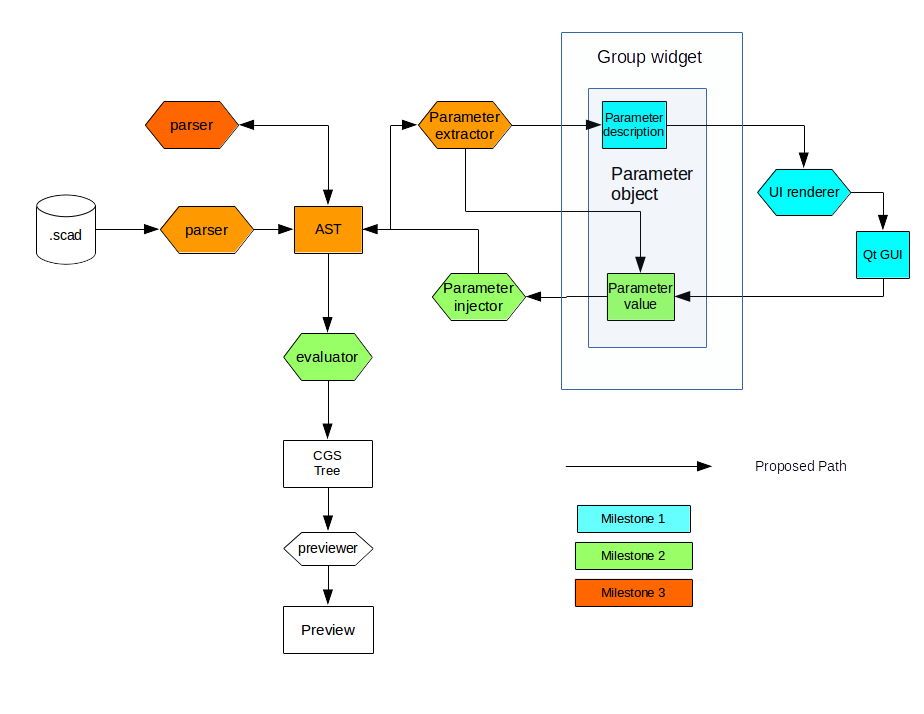
\includegraphics[width=\linewidth]{images/flowchart.png}
	\caption{Flowchart of Customizer}
	\label{fig:FD1}
\end{figure}

\subsection{Detailed Description}

The basic implementation of this project is almost done in form of prototype. There is need to modify the structure of the project. We have to divide the task into there parts:

\begin{enumerate}
	\item \textbf{Front end}
	It will deal with how the parameter will look to the user like in form of range or spinbox etc. This part will include two parts:
	\begin{enumerate}
		\item \textbf{Individual Parameter}
		This will define how individual parameters will look like
		\item \textbf{Container Widget}
		This will contain UI features common to all parameter. This widget will contain all parameter widget.
		
	\end{enumerate}
	
	\item \textbf{Back End}
	This will include the parser part that will create AST nodes and we can extract the parameters from the AST. we can use the single parser for the whole .scad file or separate parser for extracting the parameters with annotations.
	
	The Back-end part will also include the parameter extractor and injector or the injector can be included in parameter object which will serve as interface
	\item \textbf{Interface}
	This will include the parameter object which will serve as an interface between both Back end and Front end. Parameter object will contain information regarding each individual parameter like parameter name, default value, and information how this parameter will be displayed as widgets to the user. Parameter object could also include the method to inject the value of the individual parameter into the AST.
	
\end{enumerate}


\section{Dependency Graph}
A Dependency Graph is a graphical representation of the which module is dependent on which other modules. A Dependency Graph is often used as a preliminary step to creating an overview of the system. Dependency Graph also gives overview of how good is the design of the system.
OpenSCAD being were huge software it would be difficult to make the dependency graph of whole software. So, here is  Dependency Graph of Customizer is as following-:
\begin{enumerate}
\item \textbf{Dependency graph of Comment.h:} Figure \ref{fig:comment1} shows the modules on which the comment.h module is dependent.
\item \textbf{Caller graph of Comment.h:} Figure \ref{fig:comment} shows the modules that use the module comment.h.
\item \textbf{Caller graph of ParameterWidget.cc:} Figure \ref{fig:dependency} show the modules that uses the module ParameterWidget.h.
\end{enumerate}

\begin{figure}
	\centering
	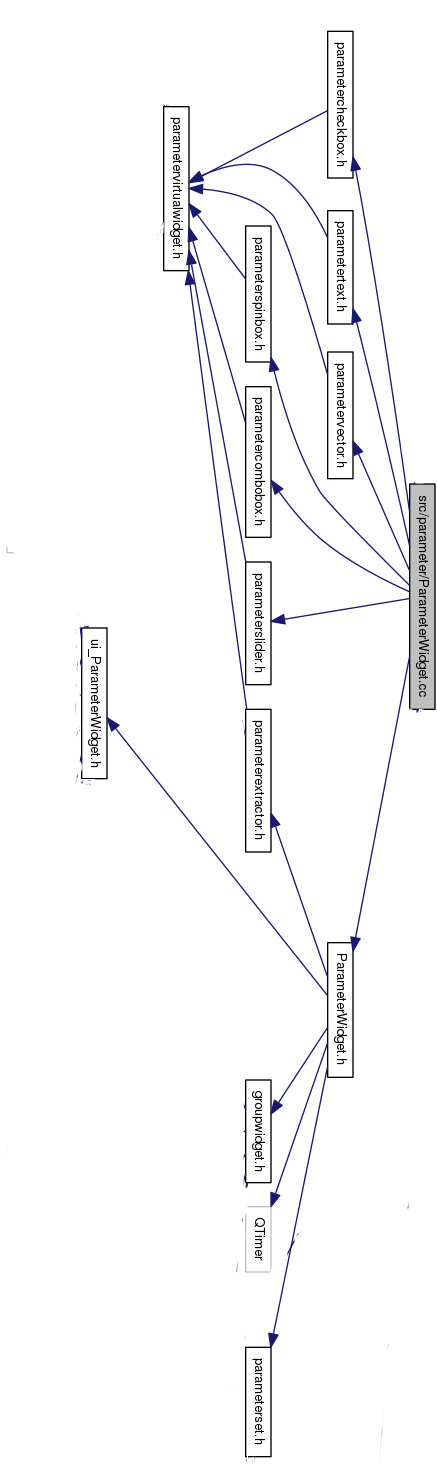
\includegraphics[width=0.7\linewidth,height=1.37\columnwidth]{images/dependene}
	\caption{ Dependency graph of Comment.h}
	\label{fig:dependency}
\end{figure}

\begin{figure}
\centering

\includegraphics[width=0.25\linewidth,height=1.37\columnwidth]{images/comment}
\caption{Caller graph of Comment.h}
\label{fig:comment}
\end{figure}
\begin{figure}
\centering
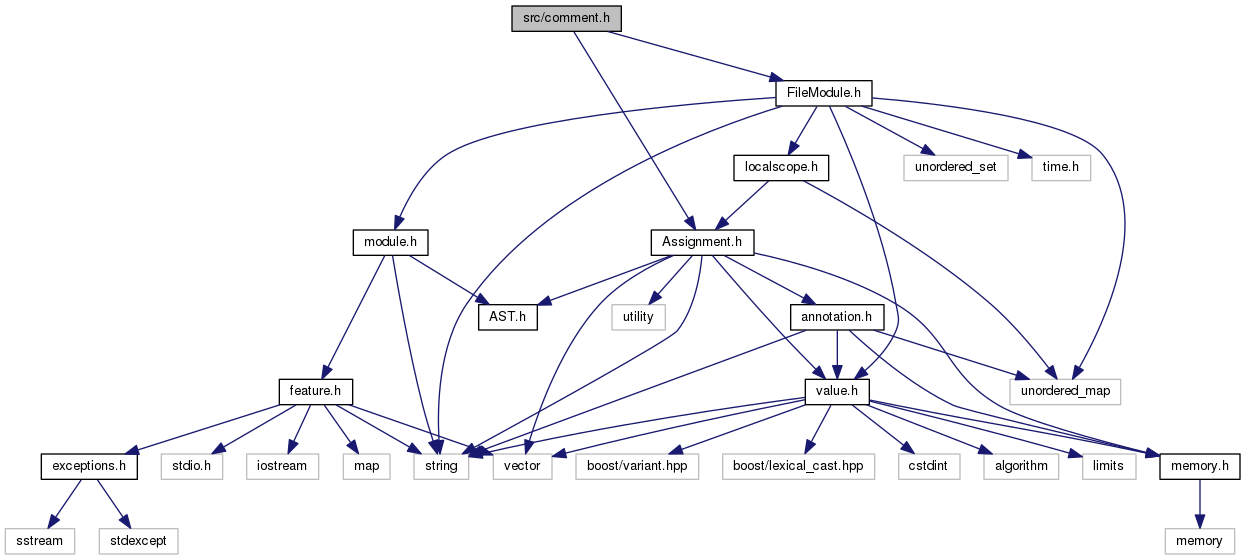
\includegraphics[width=\linewidth,height=1.35\columnwidth]{images/comment1}
\caption{Caller graph of ParameterWidget.cc}
\label{fig:comment1}
\end{figure}




\section{Class Diagrams}
Class Diagrams describe the static structure of the system. Following classes diagram represent the relationship between different classes in OpenSCAD and customizer:
\begin{enumerate}
	\item Figure \ref{fig:collaborative1} shows the class diagram of the ParameterWidgetVirtual class which is the basse class of all the Widget classes i.e ParameterCheckbox, ParameterVector,ParmeterSpinbox, ParameterComboBox,ParameterSlider, ParameterText.
	\item Figure \ref{fig:collaborative} shows the class diagram of the ParameterWidget class which is the main class for whole the Customizer GUI and also show how this class is related to various classes in custmoizer.
	
	\item Figure \ref{fig:classAnnotation__coll__graph}  shows the class diagram of the Annotation class which is the main node of the AST that support the customizer feature and also show how this class is related to various classes in the customizer.
\end{enumerate}
\begin{figure}
    \centering
    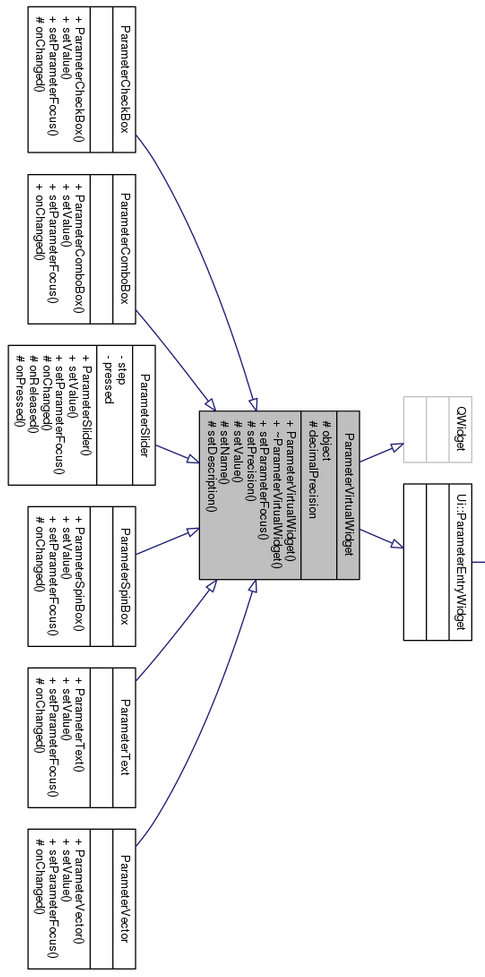
\includegraphics[width=0.5\linewidth,,height=1.38\columnwidth]{images/collaborative1}
    \caption{Class Diagram for Customizer (Part A) }
    \label{fig:collaborative1}
\end{figure}
\begin{figure}
    \centering
    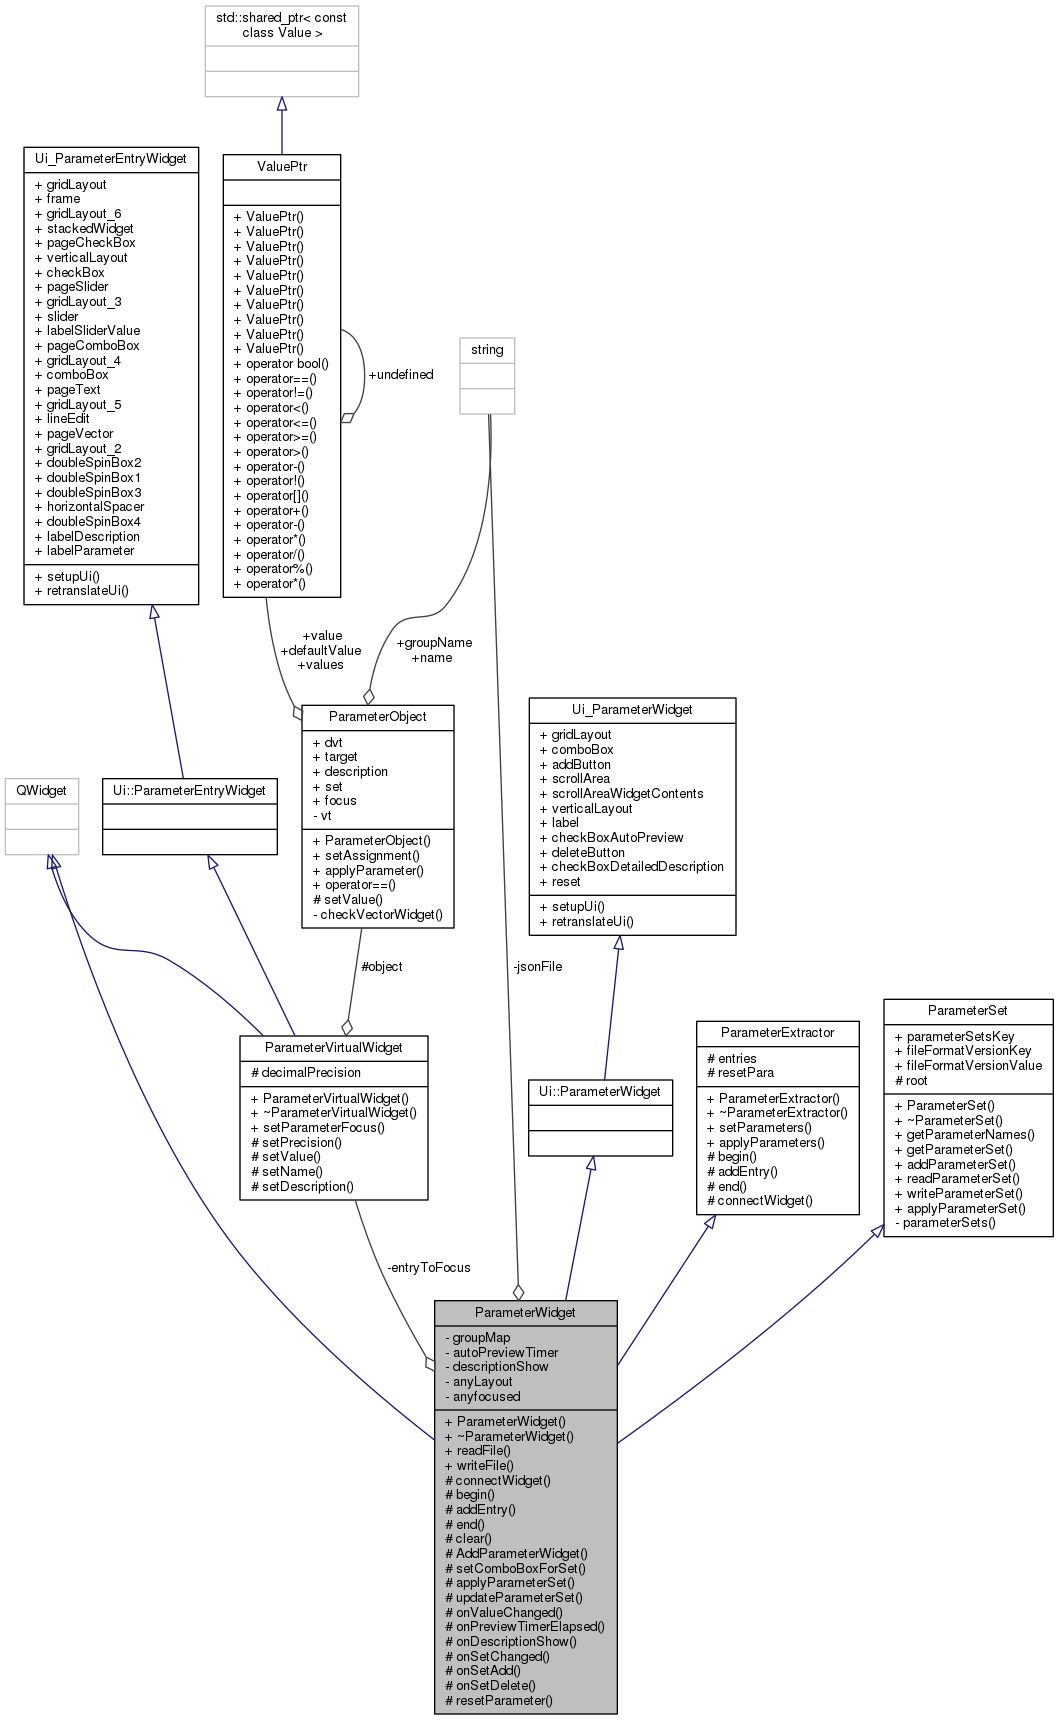
\includegraphics[scale=0.39]{images/collaborative}
    \caption{Class Diagram for Customizer (Part B)}
    \label{fig:collaborative}
\end{figure}
\begin{figure}
\centering
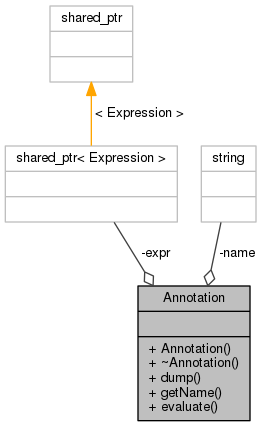
\includegraphics[width=0.4\linewidth]{images/classAnnotation__coll__graph}
\caption{Class Diagram for Annotation}
\label{fig:classAnnotation__coll__graph}
\end{figure}
\section{Dependencies}
Dependencies include softwares or framework that need to be installed for proper working of this software.

\emph{{\large There is no software dependencies to Install this software.}}

This software could be installed on any given list of operating system.

\begin{enumerate}
	\item Mac OS X
	\item Windows
	 \begin{enumerate} 
	 	\item XP or newer on x86 32/64 bit
	 \end{enumerate}
	\item Linux
	\begin{enumerate} 
		\item Debian 
		\item Ubuntu 
		\item Kubuntu
		\item Arch Linux
		\item openSUSE
		\item Fedora
	 \end{enumerate}
	\item BSD
	\begin{enumerate}
		\item NetBSD  $\geq 6.1$
		\item FreeBSD $\geq 10 $
		\item OpenBSD
	\end{enumerate}
\end{enumerate}	 
 

But If you want to build OpenSCAD this software from soucre code on \emph{any OS}, you need some libraries and tools. The version
numbers in brackets specify the versions which have been used for
development. Other versions may or may not work as well.

If you're using a newer version of Ubuntu, you can install these 
libraries from aptitude. If you're using Mac, or an older Linux/BSD, there 
are build scripts that download and compile the libraries from source. 
Follow the instructions for the platform you're compiling on below.

\begin{enumerate} 
	\item A C++ compiler supporting C++11
	
	\item Qt$  4.4 \rightarrow 5.x $ (http://qt.io/ )
	
	\item QScintilla2 $ (2.7 \rightarrow $)(http://www.riverbankcomputing.co.uk/software/qscintilla/)
	
	\item CGAL ($ 3.6 \rightarrow $) (http://www.cgal.org/)
	
	\item GMP (5.x) (http://www.gmplib.org/)
	
	\item MPFR (3.x)(http://www.mpfr.org/)
	
	\item cmake ($ 2.8 \rightarrow $, required by CGAL and the test framework))(http://www.cmake.org/)
	
	\item boost ($ 1.35 \rightarrow $) (http://www.boost.org/)
	
	\item OpenCSG ($ 1.3.2 \rightarrow $)(http://www.opencsg.org/)
	
	\item GLEW ($ 1.5.4 \rightarrow $)(http://glew.sourceforge.net/)
	
	\item Eigen (3.x)(http://eigen.tuxfamily.org/)
	
	\item glib2 (2.x)(https://developer.gnome.org/glib/)
	
	\item fontconfig ($ 2.10 \rightarrow  $)(http://fontconfig.org/)
	
	\item freetype2 ($ 2.4 \rightarrow  $)(http://freetype.org/)
	
	\item harfbuzz ($ 0.9.19 \rightarrow  $)(http://harfbuzz.org/)
	
	\item Bison ($ 2.4 \rightarrow $ )(http://www.gnu.org/software/bison/)
	
	\item Flex ($ 2.5.35 \rightarrow  $)(http://flex.sourceforge.net/)
	
	\item pkg-config ($ 0.26 \rightarrow $ )(http://www.freedesktop.org/wiki/Software/pkg-config/)
	
\end{enumerate}





\newpage
\chapter{DEVELOPMENT AND IMPLEMENTATION}
\section{C++}

\begin{figure}[h]
	\centering 
\includegraphics[scale=0.3]{images/c++.png}
	\caption{C++ Logo}
\end{figure}

C++ is a general-purpose programming language. It has imperative, object-oriented and generic programming features, while also providing facilities for low-level memory manipulation.

It was designed with a bias toward system programming and embedded, resource-constrained and large systems, with performance, efficiency and flexibility of use as its design highlights. C++ has also been found useful in many other contexts, with key strengths being software infrastructure and resource-constrained applications, including desktop applications, servers (e.g. e-commerce, web search or SQL servers), and performance-critical applications (e.g. telephone switches or space probes). C++ is a compiled language, with implementations of it available on many platforms and provided by various organizations, including the Free Software Foundation (FSF's GCC), LLVM, Microsoft, Intel and IBM.

C++ is standardized by the International Organization for Standardization (ISO), with the latest standard version ratified and published by ISO in December 2014 as ISO/IEC 14882:2014 (informally known as C++14). The C++ programming language was initially standardized in 1998 as ISO/IEC 14882:1998, which was then amended by the C++03, ISO/IEC 14882:2003, standard. The current C++14 standard supersedes these and C++11, with new features and an enlarged standard library. Before the initial standardization in 1998, C++ was developed by Bjarne Stroustrup at Bell Labs since 1979, as an extension of the C language as he wanted an efficient and flexible language similar to C, which also provided high-level features for program organization.

Many other programming languages have been influenced by C++, including C\#, D, Java, and newer versions of C (after 1998).

Features of Language:
\begin{enumerate}
	\item Object storage
	\begin{enumerate}
		\item Static storage duration objects
		\item Thread storage duration objects
		\item Automatic storage duration objects
		\item Dynamic storage duration objects
	\end{enumerate}
	\item Templates
	\item Objects
	\begin{enumerate}
		\item Encapsulation
		\item Inheritance
	\end{enumerate}
	\item Operators and operator overloading
	\item Polymorphism
	\begin{enumerate}
		\item Static polymorphism
		\item Dynamic polymorphism
		\begin{enumerate}
			\item Inheritance
			\item Virtual member functions
		\end{enumerate}
	\end{enumerate}
\item Lambda expressions
\item Exception handling
\end{enumerate}
\section{Flex}

Flex (fast lexical analyzer generator) is a free and open-source software alternative to lex. It is a computer program that generates lexical analyzers (also known as "scanners" or "lexers"). It is frequently used as the lex implementation together with Berkeley Yacc parser generator on BSD-derived operating systems (as both lex and yacc are part of POSIX), or together with GNU bison (a version of yacc) in *BSD ports and in GNU/Linux distributions. Unlike Bison, flex is not part of the GNU Project and is not released under the GNU Public License.

Flex was written in C by Vern Paxson around 1987. He was translating a Ratfor generator, which had been led by Jef Poskanzer

Input to Lex is divided into three sections with \%\% dividing the sections. Flex .l specification file:
\begin{verbatim}
	/*** Definition section ***/
	
	%%
	
	/*** Rules section ***/
	
	%%
	
	/*** C Code section ***/
\end{verbatim}

\section{Bison}

\begin{figure}[h]
	\centering 
\includegraphics[scale=0.2]{images/gnu.png}
	\caption{GNU Logo}
\end{figure}

Bison is a general-purpose parser generator that converts an annotated context-free grammar into a deterministic LR or generalized LR (GLR) parser employing LALR(1) parser
tables.
Once you are proficient with Bison, you can use it to develop a wide range of language parsers, from those used in simple desk calculators to complex programming languages.


Bison is upward compatible with Yacc: all properly-written Yacc grammars ought to work with Bison with no change. Anyone familiar with Yacc should be able to use Bison with little trouble. You need to be fluent in C or C++ programming in order to use Bison
or to understand this manual. Java is also supported as an experimental feature.


Bison was written originally by Robert Corbett. Richard Stallman made it Yacc-compatible. Wilfred Hansen of Carnegie Mellon University added multi-character string literals and other features. Since then, Bison has grown more robust and evolved many
other new features thanks to the hard work of a long list of volunteers.

Bison .y specification file:

\begin{verbatim}
	/*** Definition section ***/
	
	%%
	
	/*** Rules section ***/
	
	%%
	
	/*** C Code section ***/

\end{verbatim}
\section{Qt}

\begin{figure}[h]
	\centering 
\includegraphics[scale=0.1]{images/qt.png}
	\caption{Qt Logo}
\end{figure}

Qt is a cross-platform application framework that is widely used for developing application software that can be run on various software and hardware platforms with little or no change in the underlying codebase, while still being a native application with native capabilities and speed. Qt is currently being developed both by The Qt Company, a company listed on the Nasdaq Helsinki Stock Exchange and the Qt Project under open-source governance, involving individual developers and firms working to advance Qt. Qt is available with both commercial and open source GPL 2.0, GPL 3.0, and LGPL 3.0 licenses.

Qt is used mainly for developing application software with graphical user interfaces (GUIs); however, programs without a GUI can be developed, such as command-line tools and consoles for servers. An example of a non-GUI program using Qt is the Cutelyst web framework. GUI programs created with Qt can have a native-looking interface, in which case Qt is classified as a widget toolkit.

Qt uses standard C++ with extensions including signals and slots that simplify handling of events, and this helps in development of both GUI and server applications which receive their own set of event information and should process them accordingly. Qt supports many compilers, including the GCC C++ compiler and the Visual Studio suite. Qt also provides Qt Quick, that includes a declarative scripting language called QML that allows using JavaScript to provide the logic. With Qt Quick, rapid application development for mobile devices became possible, although logic can be written with native code as well to achieve the best possible performance. Qt can be used in several other programming languages via language bindings. It runs on the major desktop platforms and some of the mobile platforms. It has extensive internationalization support. Non-GUI features include SQL database access, XML parsing, JSON parsing, thread management and network support.

%\input{input/Development/make.tex}
%\input{input/Development/ctest.tex}
%\input{input/Development/travis.tex}
\section{Introduction to \LaTeX}

\LaTeX, I had never heard about this term before doing this project,
but when I came to know about it's features, found it excellent. 
\LaTeX{} (pronounced /ˈleɪtɛk/, /ˈleɪtɛx/, /ˈlɑːtɛx/, or /ˈlɑːtɛk/) is a 
document markup language and document preparation system for the \TeX{} 
typesetting  program. Within the typesetting system, its name is styled 
as \LaTeX.

\image{0.9}{images/donald.png}{Donald Knuth, Inventor Of \TeX{} 
typesetting system}

Within the typesetting system, its name is styled as \LaTeX. The term 
\LaTeX{} refers only to the language in which documents are written, 
not to the editor used to write those documents. In order to create a 
document in \LaTeX, a .tex file must be created using some form of text 
editor. While most text editors can be used to create a \LaTeX{} document, 
a number of editors have been created specifically for working with \LaTeX.

\LaTeX{} is most widely used by mathematicians, scientists, 
engineers, philosophers, linguists, economists and other scholars in 
academia. As a primary or intermediate format, e.g., translating DocBook 
and other XML-based formats to PDF, \LaTeX{} is used because of the 
high quality of typesetting achievable by \TeX. The typesetting system 
offers programmable desktop publishing features and extensive facilities 
for automating most aspects of typesetting and desktop publishing, 
including numbering and cross-referencing, tables and figures, 
page layout and bibliographies.

\LaTeX{} is intended to provide a high-level language that
accesses the power of \TeX. \LaTeX{} essentially comprises a
collection of \TeX{} macros and a program to process \LaTeX documents. 
Because the \TeX{} formatting commands are very low-level, it is usually 
much simpler for end-users to use \LaTeX{}.


\subsection{Typesetting}
\LaTeX{} is based on the idea that authors should be able to focus on 
the content of what they are writing without being distracted by its 
visual presentation. In preparing a \LaTeX{} document, the author 
specifies the logical structure using familiar concepts such as 
chapter, section, table, figure, etc., and lets the \LaTeX{} system 
worry about the presentation of these structures. It therefore 
encourages the separation of layout from content while still allowing 
manual typesetting adjustments where needed. 

\begin{verbatim}
\documentclass[12pt]{article}
\usepackage{amsmath}
\title{\LaTeX}
\date{}
\begin{document}
  \maketitle 
  \LaTeX{} is a document preparation system 
  for the \TeX{} typesetting program.
   \par 
   $E=mc^2$
\end{document}
\end{verbatim}


\section{Introduction to Doxygen}
\begin{figure}[h]
\centering 
\includegraphics[scale=1.3]{images/Doxygen.png}
\caption{Doxygen Logo}
\end{figure}
\noindent Doxygen is a documentation generator, a tool for writing software reference 
documentation. The documentation is written within code, and is thus 
relatively easy to keep up to date. Doxygen can cross reference 
documentation and code, so that the reader of a document can easily 
refer to the actual code.

Doxygen supports multiple programming languages, especially C++, C, 
C\#, Objective-C, Java, Python, IDL, VHDL, Fortran and PHP.[2] Doxygen
 is free software, released under the terms of the GNU General Public 
License.\\

\subsection{Features of Doxygen}
\begin{itemize}
\item Requires very little overhead from the writer of the documentation. 
Plain text will do, Markdown is support, and for more fancy or structured 
output HTML tags and/or some of doxygen's special commands can be used.
\item Cross platform: Works on Windows and many Unix flavors (including 
Linux and Mac OS X).
\item Comes with a GUI frontend (Doxywizard) to ease editing the options 
and run doxygen. The GUI is available on Windows, Linux, and Mac OS X.
\item Automatically generates class and collaboration diagrams in HTML 
(as clickable image maps) and $\mbox{\LaTeX}$ (as Encapsulated PostScript 
images).
\item Allows grouping of entities in modules and creating a hierarchy 
of modules.
\item Doxygen can generate a layout which you can use and edit to change 
the layout of each page.
\item Can cope with large projects easily.
\end{itemize}
\subsection{Installation of Doxygen}
Doxygen can be installed using following commands:\\

\hspace{4pt} \$ git clone https://github.com/doxygen/doxygen.git

\hspace{4pt} \$ cd doxygen

\hspace{4pt} \$ ./configure

\hspace{4pt} \$ make

\begin{figure}[H]
\centering 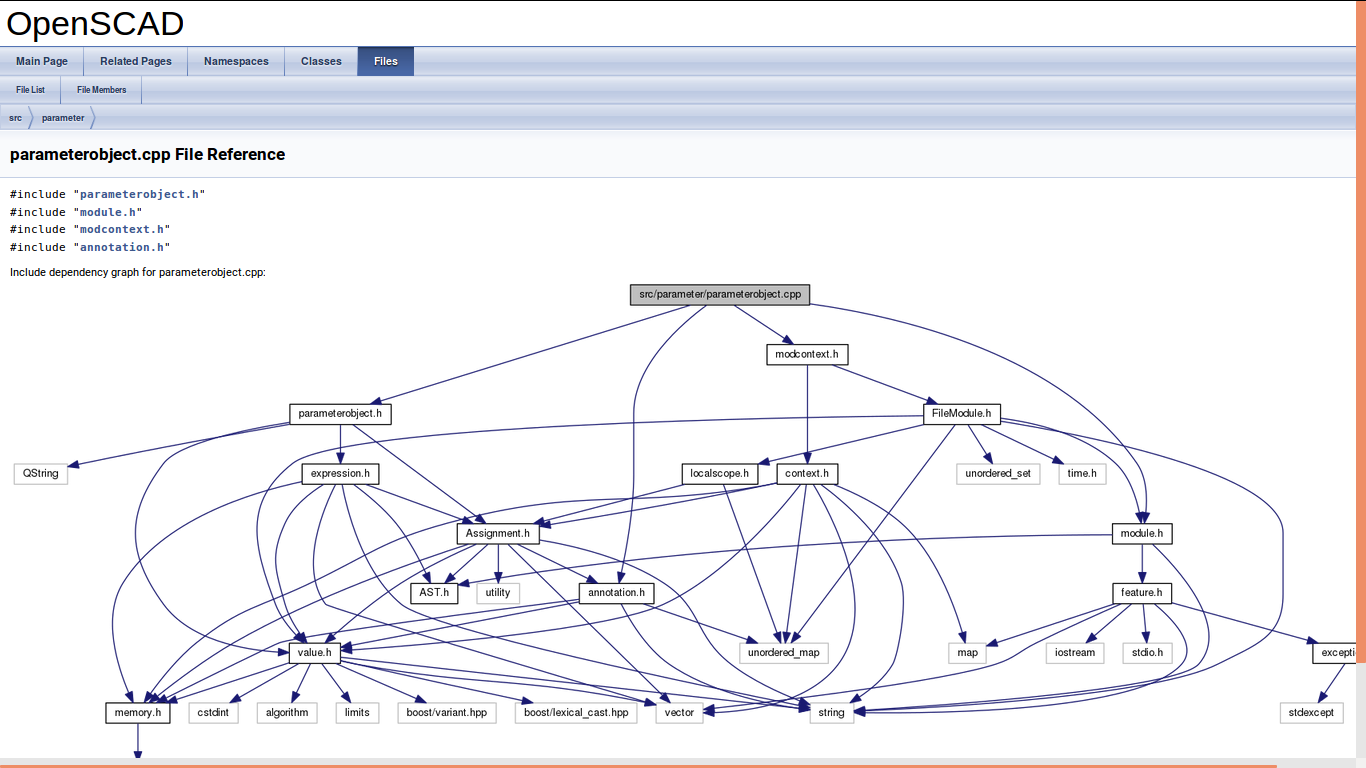
\includegraphics[scale=.35]{images/doc.png}
\caption{Documentation using Doxygen (main page)}
\end{figure}


\begin{figure}[H]
\centering 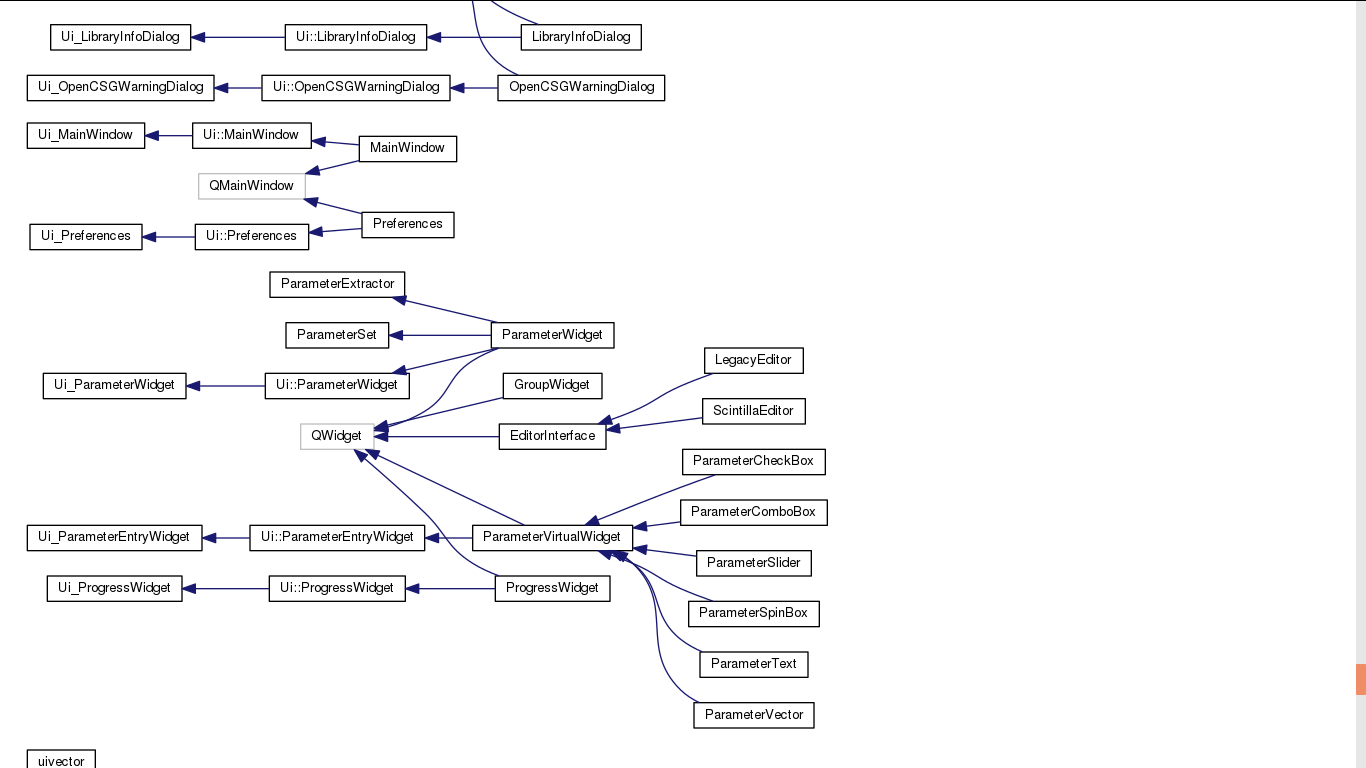
\includegraphics[scale=.35]{images/doc1.png}
\caption{Doxygen documentation of a function}
\end{figure}
\begin{figure}[H]
\centering 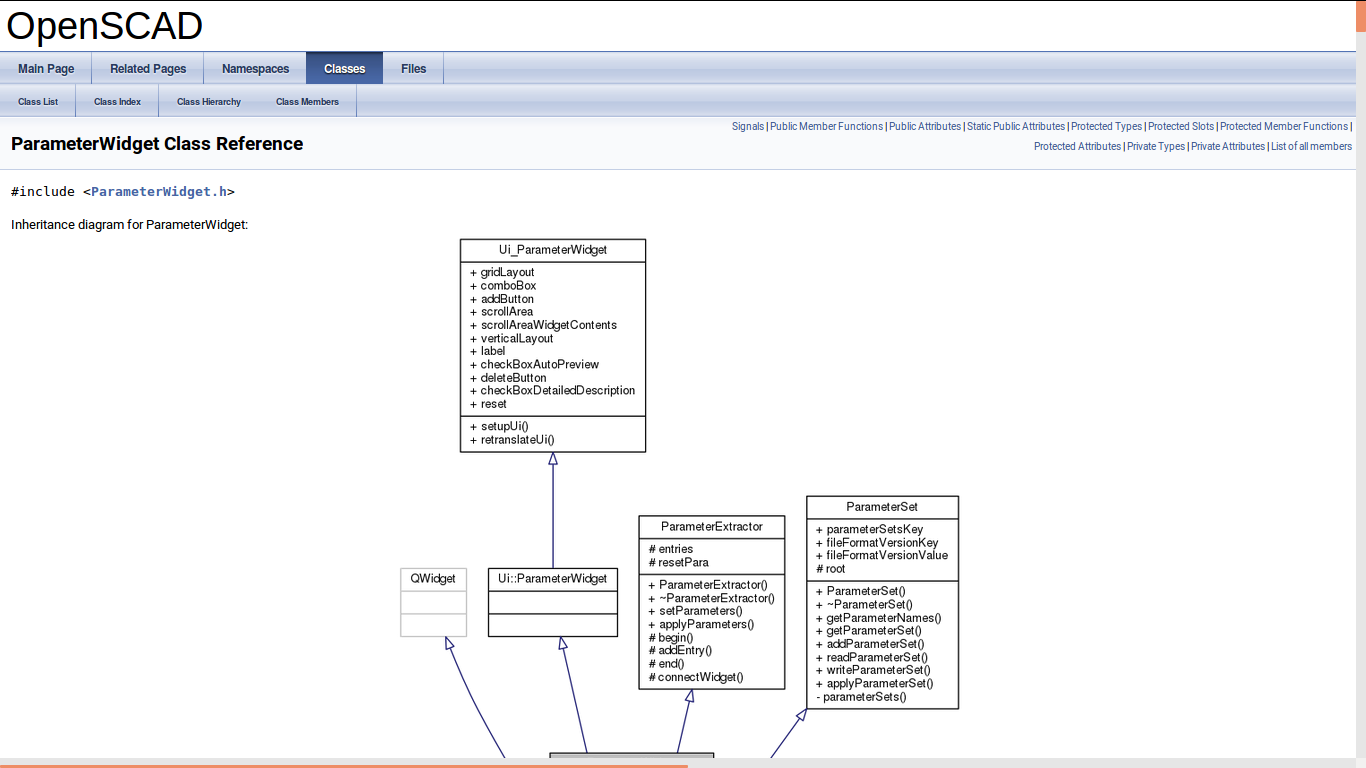
\includegraphics[scale=.35]{images/doc2.png}
\caption{Documentation using Doxygen(list of files)}
\end{figure}




\section{Introduction to Github}
\begin{figure}[!ht]
\centering

\includegraphics[width=0.3\textwidth]{images/github.png}                   
\caption{Github Logo}
\hspace{-1.5em}
\end{figure}
\leavevmode\\
GitHub is a Git repository web-based hosting service which offers all of the functionality of Git as well as adding many of its own features. Unlike Git which is strictly a command-line tool, Github provides a web-based graphical interface and desktop as well as mobile integration. It also provides access control and several collaboration features such as wikis, task management, and bug tracking and feature requests for every project.\\

GitHub has become such a staple amongst the open-source development community that many developers have begun considering it a replacement for a conventional resume and some employers require applications to provide a link to and have an active contributing GitHub account in order to qualify for a job.\\

The Git feature that really makes it stand apart from nearly every
other Source Code Management (SCM) out there is its branching model.\\
\\
Git allows and encourages you to have multiple local branches that can
be entirely independent of each other. The creation, merging, and
deletion of those lines of development takes seconds.\\ \\
This means that you can do things like:
\begin{itemize}
\item Frictionless Context Switching.\\ Create a branch to try out an
idea, commit a few times, switch back to where you branched from,
apply a patch, switch back to where you are experimenting, and merge
it in.
\item Role-Based Code lines. \\ Have a branch that always contains only
what goes to production, another that you merge work into for testing,
and several smaller ones for day to day work.
\item Feature Based Work flow. \\ Create new branches for each new
feature you're working on so you can seamlessly switch back and forth
between them, then delete each branch when that feature gets merged
into your main line.
\item Disposable Experimentation.\\  Create a branch to experiment in,
realize it's not going to work, and just delete it - abandoning the
work—with nobody else ever seeing it (even if you've pushed other
branches in the meantime).
\end{itemize}
Notably, when you push to a remote repository, you do not have to push
all of your branches. You can choose to share just one of your
branches, a few of them, or all of them. This tends to free people to
try new ideas without worrying about having to plan how and when they
are going to merge it in or share it with others.\\ \\
There are ways to accomplish some of this with other systems, but the
work involved is much more difficult and error-prone. Git makes this
process incredibly easy and it changes the way most developers work
when they learn it.

\subsection{What is Git?}
\begin{figure}[!ht]
\centering

\includegraphics[width=0.3\textwidth]{images/git.png}                   
\caption{Git Logo}
\hspace{-1.5em}
\end{figure}
Git is a distributed revision control and source code management (SCM) system with an emphasis on speed, data integrity, and support for distributed, non-linear workflows. Git was initially designed and developed by Linus Torvalds for Linux kernel development in 2005, and has since become the most widely adopted version control system for software development.\\

As with most other distributed revision control systems, and unlike most client–server systems, every Git working directory is a full-fledged repository with complete history and full version-tracking capabilities, independent of network access or a central server. Like the Linux kernel, Git is free and open source software distributed under the terms of the GNU General Public License version 2 to handle everything from small to very large projects with speed and efficiency.\\

Git is easy to learn and has a tiny footprint with lightning fast performance. It outclasses SCM tools like Subversion, CVS, Perforce, and ClearCase with features like cheap local branching, convenient staging areas, and multiple workflows.\\


\subsection{Various Git Commands}

Git is the open source distributed version control system that facilitates GitHub activities on your laptop or desktop. The commonly used Git command line instructions are:-\\

\begin{description}

\item [\$ git init [ project-name]]\\
Creates a new local repository with the specified name
\item [\$ git clone [url]]\\
Downloads a project and its entire version history\\
\item [\$ git merge [bookmark]/[branch]]\\
Combines bookmark’s branch into current local branch

\item [\$ git push [alias][branch]]\\
Uploads all local branch commits to GitHub

\item [\$ git pull] \leavevmode \\
Downloads bookmark history and incorporates changes

\item [\$ git add [file]]\\
Snapshots the file in preparation for versioning

\item [\$ git reset [file]]\\
Unstages the file, but preserve its contents

\item [\$ git commit -m "[descriptive message]"]\\
Records file snapshots permanently in version history\\

\end{description}

\section{Implementation}
\subsection{Customizer}

\begin{figure}
	\centering 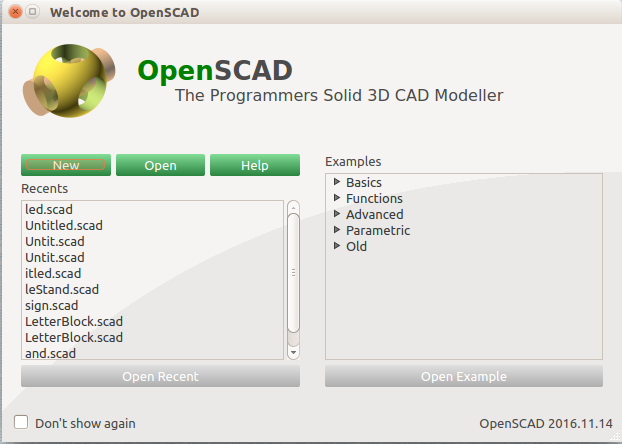
\includegraphics[scale=0.60]{images/output/1.png}
	\caption{StartUp Screen for OpenSCAD}
	\label{fig:1}
\end{figure}

Customizer  will provide User Interface to Customize Models interactively instead of modifying them manually. It will make the user able to create the templates for given model which can further be customized to cater to their need of different users and also provide a feature to save the set of parameters which define a different model using the same template of the model.
\subsection{Activation of Customizer functions}
\begin{itemize}
	
	\item This is experimental functionality.So, Initially
	OpenSCAD will look like \ref{fig:Normal OpenSCAD}
	\item In [Edit] menu, select [Preferencews] then open tab [Features], tick Customizer, then close the window when tick shown \ref{fig:3}.
	\item In View menu, you shall now have an option [Hide customizer], that you shall untick. Then you will be able to see the customizer \ref{fig:OpenSCAD with Customizer}
	
\end{itemize}

\begin{figure}
	\centering 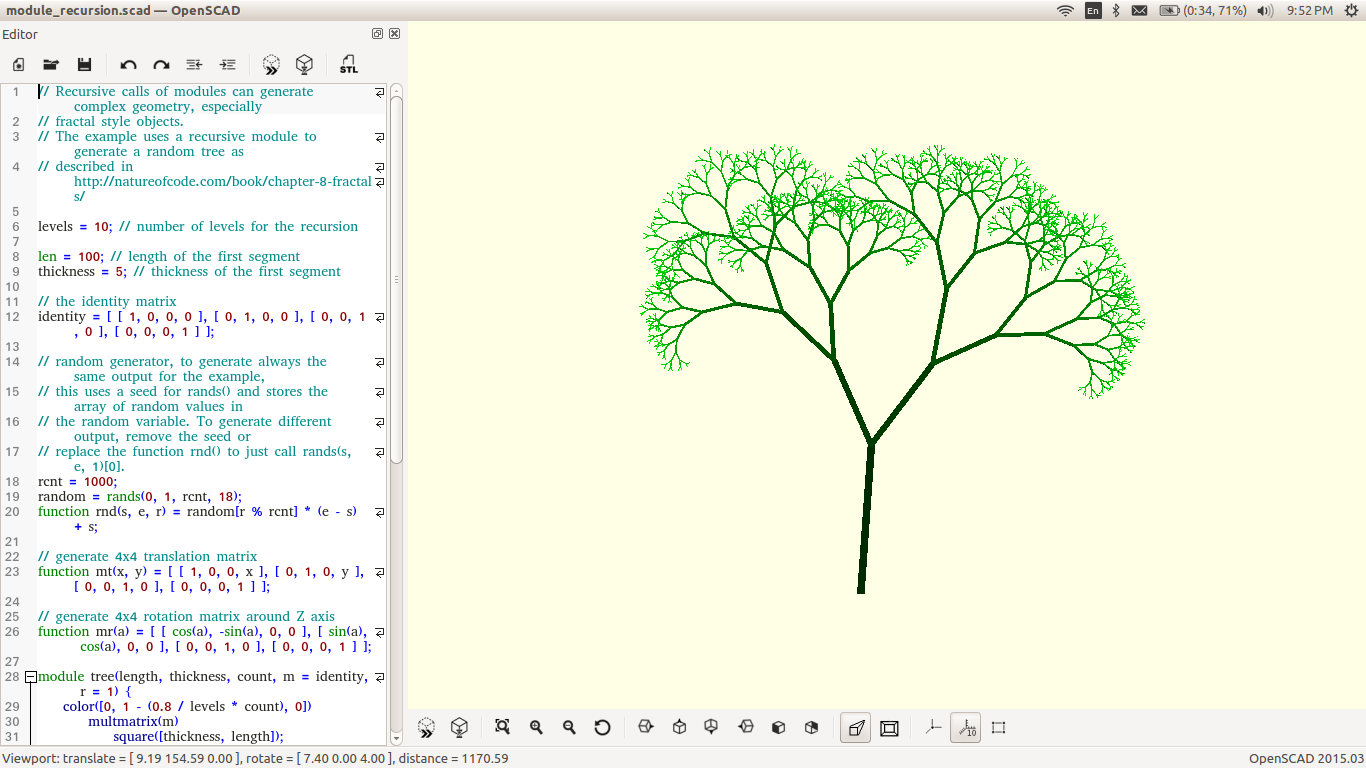
\includegraphics[width=\linewidth]{images/output/2.png}
	\caption{OpenSCAD without customizer}
	\label{fig:Normal OpenSCAD}
\end{figure}
\begin{figure}
	\centering 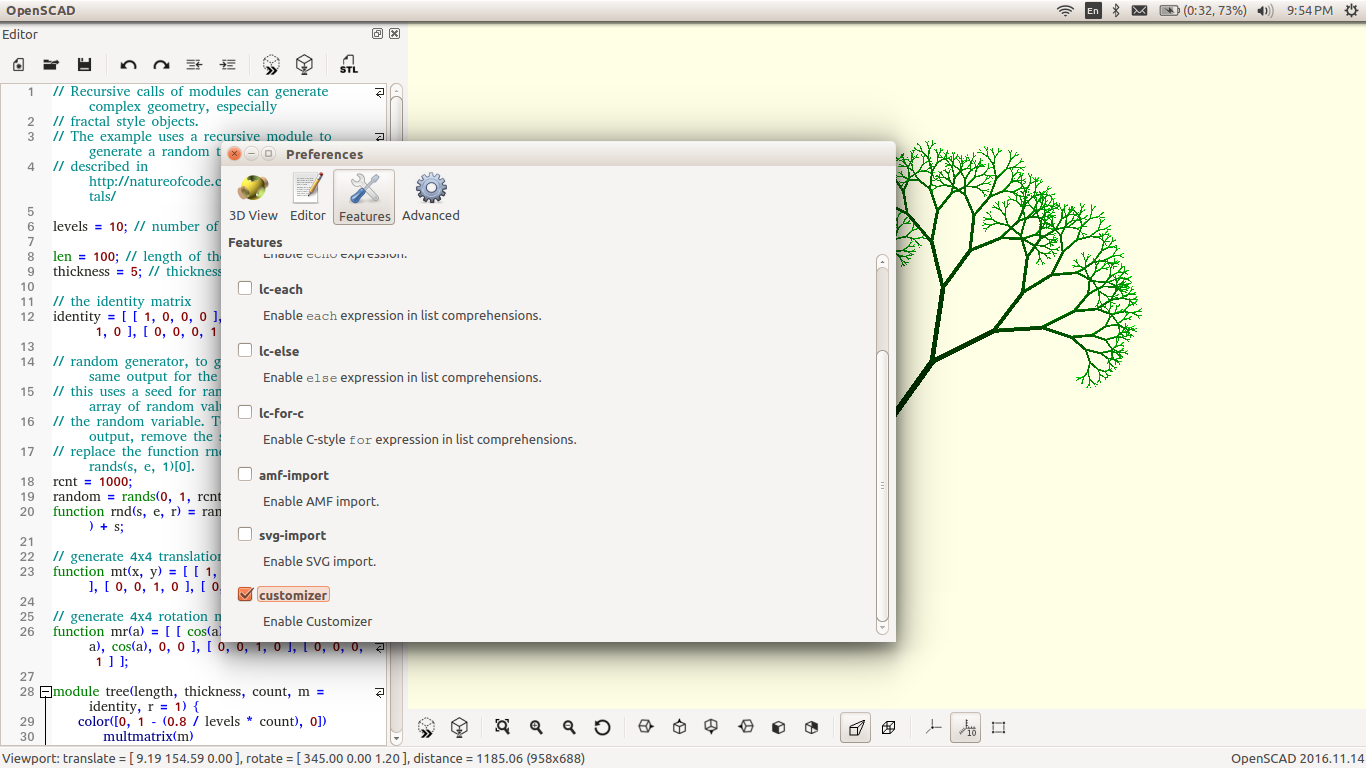
\includegraphics[width=\linewidth]{images/output/3.png}
	\caption{Preferences Widget to activate Customizer}
	\label{fig:3}
\end{figure}
\begin{figure}
	\centering 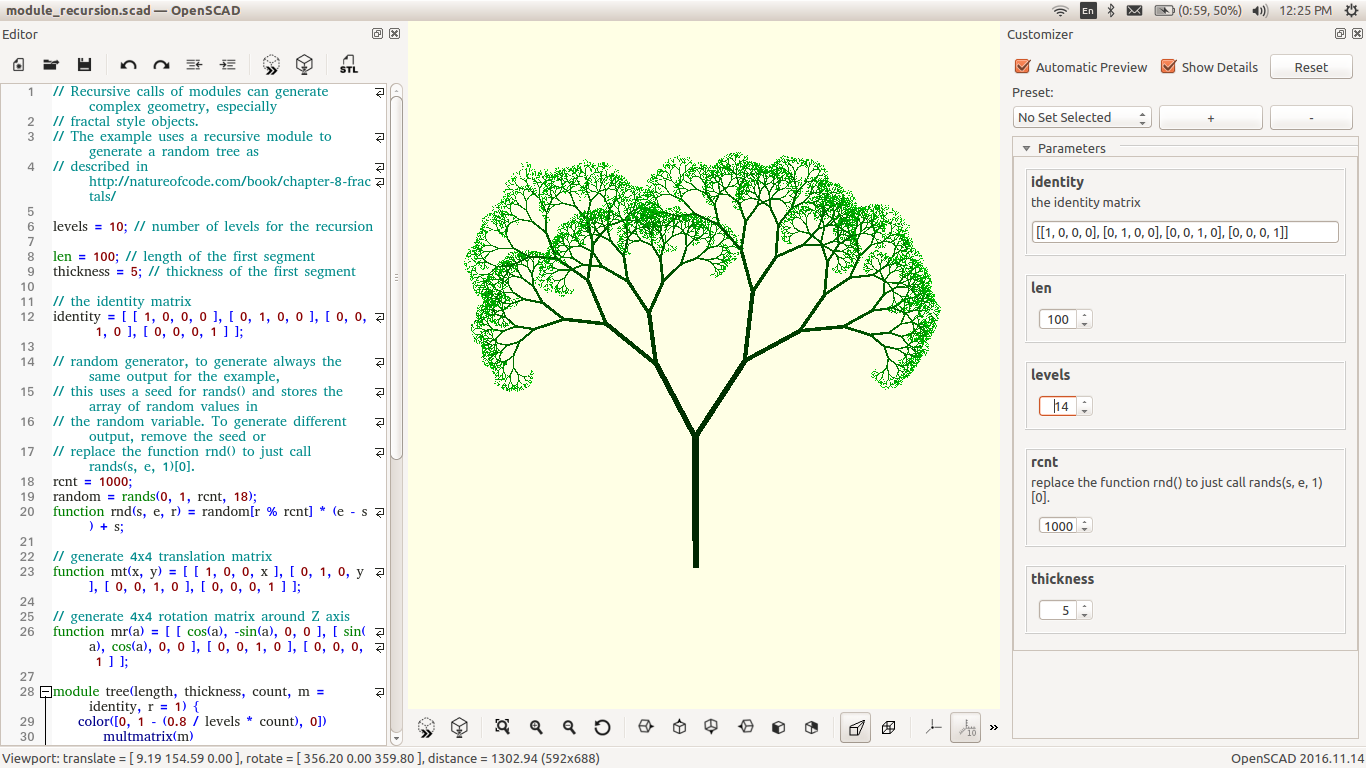
\includegraphics[width=\linewidth]{images/output/5.png}
	\caption{OpenSCAD with Customizer }
	\label{fig:OpenSCAD with Customizer}
\end{figure}

\subsection{Syntax support for generation of the customization form}

\begin{lstlisting}[language=c++]
// variable description
variable name = defaultValue; // possible values
\end{lstlisting}

Parameter will be decorated with meta data using the comments and the single line comments above the parameter could be used to describe the meaning of the parameter and its use. The comments in same line as that of parameter is used to define the GUI that have to be used to modify that values of that parameter.

Following is the syntax for how to define different types of widgets in the form

\begin{enumerate}
	\item \textbf{Drop down box:} \ref{fig:example} Following type of comboBox could be created with following syntax:
	\begin{figure}
		\centering
		\includegraphics[width=\linewidth]{images/example}
		\caption{Shows the different types ComboBox, Slider}
		\label{fig:example}
	\end{figure}
	
	\begin{lstlisting}[language=c++]
	// combo box for nunber
	Numbers=2; // [0, 1, 2, 3]
	
	// combo box for string
	Strings="foo"; // [foo, bar, baz]
	
	//labeled combo box for numbers
	Labeled_values=10; // [10:L, 20:M, 30:L]
	
	//labeled combo box for string
	Labeled_value="S"; // [S:Small, M:Medium, L:Large]
	\end{lstlisting}
	\item \textbf{Slider:} Only numbers are allowed in this one, \ref{fig:example} specify any of the following:
	\begin{lstlisting}[language=c++]
	// slider widget for number
	slider =34; // [10:100]
	
	//step slider for number
	stepSlider=2; //[0:5:100]
	\end{lstlisting}
	\item \textbf{Checkbox:} \ref{fig:example1} Following widget is created with given syntax:
	\begin{lstlisting}[language=c++]
	//description
	Variable = true;
	\end{lstlisting}
	\item \textbf{Spinbox:} \ref{fig:example1} Following widget is created with given syntax:
	\begin{lstlisting}[language=c++]
	// spinbox with step size 1
	Spinbox= 5;
	
	// spinbox with step size 0.01
	Spinbox= 5.11;
	
	//spinbox with given step size
	SpinboxWithStep= 5; //2
	\end{lstlisting}
	\item \textbf{Textbox:} \ref{fig:example1} Following widget is created with given syntax:
	\begin{lstlisting}[language=c++]
	//Text box for vector with more than 4 elements
	Vector=[12,34,44,43,23,23];
	
	// Text box for string
	String="hello";
	
	\end{lstlisting}
	\item \textbf{Special vector:} \ref{fig:example1} Following widget is created with given syntax:
	\begin{lstlisting}[language=c++]
	
	//Text box for vector with less than or equal to 4 elements
	Vector2=[12,34,45,23];
	\end{lstlisting}
	\begin{figure}
		\centering
		\includegraphics[width=\linewidth]{images/example1}
		\caption{Shows the CheckBox, TextBox, SpinBox, VectorWidget}
		\label{fig:example1}
	\end{figure}
	
\end{enumerate}

\subsection{Creating Tabs}
Parameters can be grouped into \textbf{tabs}. This feature will allow us to separate similar and related parameters. The syntax for this is also mainly similar to that of Thingiverse syntax for creating the tabs. To create a tab, use a multi-line block comment like this:

\textbf{/* [Tab Name] */}


Screenshot number \ref{fig:5} Shows the implemenation of this feature.

The following tab names are reserved for special functionality:
\begin{description}
	\item [Global] Parameters in the global tab will always be shown on every tab no matter which tab is selected. Note: there will be no tab for “Global” params, they will just always be shown in all the tabs.
	
	\item [Hidden] Parameters in the hidden tab will never be displayed. Not even the tab will be shown. Even though the variables who have not been parameterized using the Thingiverse or native syntax will not be displayed in OpenSCAD parameter widget but we have implemented this to make our comment like syntax similar as that of Thingiverse.
\end{description}

Also, the parameters who are under no tab will be displayed under TAB named “parameters”.
\begin{lstlisting}[language=c++]
// combo box for nunber
Numbers=2; // [0, 1, 2, 3]

// combo box for string
Strings="foo"; // [foo, bar, baz]


/*[ Slider ]*/
// slider widget for number
slider =34; // [10:100]

//step slider for number
stepSlider=2; //[0:5:100]

/* [Global] */

//description
Variable = true;

/*[Hidden] */

// spinbox with step size 1
Spinbox = 5;

/* [Textbox] */

//Text box for vector with more than 4 elements
Vector=[12,34,44,43,23,23];

// Text box for string
String="hello";

\end{lstlisting}

\begin{figure}
	\centering 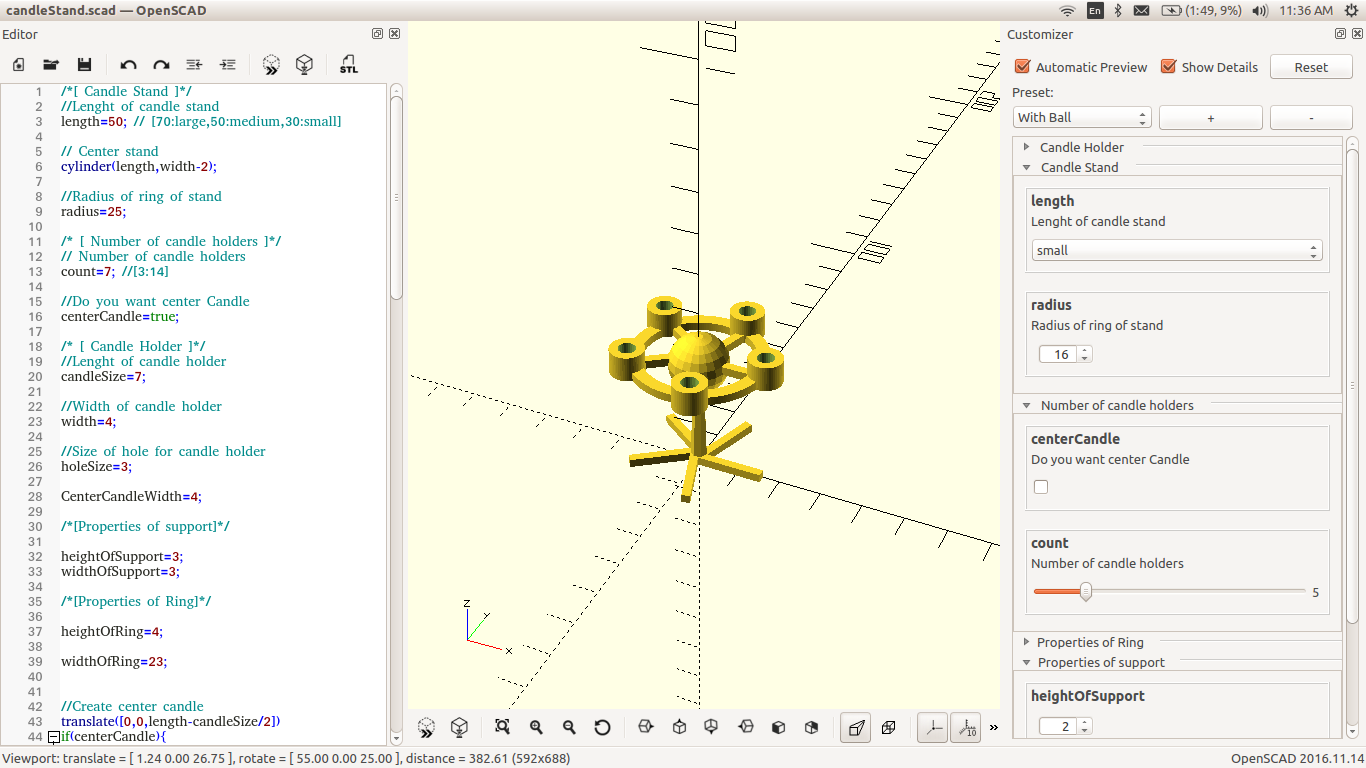
\includegraphics[width=\linewidth]{images/output/6.png}
	\caption{Shows different groups generated through customzier}
	\label{fig:5}
\end{figure}

\begin{thebibliography}{9}
\bibitem{} Dynamics of Structure(DoS), https://github.com/amarjeetkapoor1/CivilOctave
\bibitem{} \LaTeX{} https://www.sharelatex.com
\bibitem{} Sagemath www.sagemath.org/
\bibitem{} Django https://docs.djangoproject.com/
\bibitem{} Doxygen www.doxygen.org
\bibitem{} My Blog, https://amarjeetkapoor1.wordpress.com
\bibitem{} My Github Profile, https://github.com/amarjeetkapoor1
https://en.wikipedia.org/wiki/OpenSCAD
http://www.openscad.org/
http://customizer.makerbot.com/docs
https://amarjeetkapoor1.wordpress.com/2016/07/04/user-interface-for-customizing-models/
%http://www.openscad.org/news.html#20160714


logo

https://www.quora.com/Is-there-an-official-C++-logo

%https://en.wikipedia.org/wiki/GNU#/media/File:Heckert_GNU_white.svg

%https://en.wikipedia.org/wiki/Qt_(software)#/media/File:Qt_logo_2015.svg

%https://upload.wikimedia.org/wikipedia/commons/c/ce/Doxygen.png

%https://en.wikipedia.org/wiki/GitHub#/media/File:GitHub_logo_2013_padded.svg

%https://en.wikipedia.org/wiki/Git#/media/File:Git-logo.svg

%Published by the Free Software Foundation
%51 Franklin Street, Fifth Floor
%Boston, MA 02110-1301 USA
%Printed copies are available from the Free Software Foundation.
%ISBN 1-882114-44-2

%https://en.wikipedia.org/wiki/Qt_(software)

%https://en.wikipedia.org/wiki/C%2B%2B

%Flex/Bison Tutorial
%Aaron Myles Landwehr
%aron+ta@udel.edu

\end{thebibliography}



\end{document}

